\documentclass{beamer}\usepackage[]{graphicx}\usepackage[]{color}
%% maxwidth is the original width if it is less than linewidth
%% otherwise use linewidth (to make sure the graphics do not exceed the margin)
\makeatletter
\def\maxwidth{ %
  \ifdim\Gin@nat@width>\linewidth
    \linewidth
  \else
    \Gin@nat@width
  \fi
}
\makeatother

\definecolor{fgcolor}{rgb}{0.345, 0.345, 0.345}
\newcommand{\hlnum}[1]{\textcolor[rgb]{0.686,0.059,0.569}{#1}}%
\newcommand{\hlstr}[1]{\textcolor[rgb]{0.192,0.494,0.8}{#1}}%
\newcommand{\hlcom}[1]{\textcolor[rgb]{0.678,0.584,0.686}{\textit{#1}}}%
\newcommand{\hlopt}[1]{\textcolor[rgb]{0,0,0}{#1}}%
\newcommand{\hlstd}[1]{\textcolor[rgb]{0.345,0.345,0.345}{#1}}%
\newcommand{\hlkwa}[1]{\textcolor[rgb]{0.161,0.373,0.58}{\textbf{#1}}}%
\newcommand{\hlkwb}[1]{\textcolor[rgb]{0.69,0.353,0.396}{#1}}%
\newcommand{\hlkwc}[1]{\textcolor[rgb]{0.333,0.667,0.333}{#1}}%
\newcommand{\hlkwd}[1]{\textcolor[rgb]{0.737,0.353,0.396}{\textbf{#1}}}%

\usepackage{framed}
\makeatletter
\newenvironment{kframe}{%
 \def\at@end@of@kframe{}%
 \ifinner\ifhmode%
  \def\at@end@of@kframe{\end{minipage}}%
  \begin{minipage}{\columnwidth}%
 \fi\fi%
 \def\FrameCommand##1{\hskip\@totalleftmargin \hskip-\fboxsep
 \colorbox{shadecolor}{##1}\hskip-\fboxsep
     % There is no \\@totalrightmargin, so:
     \hskip-\linewidth \hskip-\@totalleftmargin \hskip\columnwidth}%
 \MakeFramed {\advance\hsize-\width
   \@totalleftmargin\z@ \linewidth\hsize
   \@setminipage}}%
 {\par\unskip\endMakeFramed%
 \at@end@of@kframe}
\makeatother

\definecolor{shadecolor}{rgb}{.97, .97, .97}
\definecolor{messagecolor}{rgb}{0, 0, 0}
\definecolor{warningcolor}{rgb}{1, 0, 1}
\definecolor{errorcolor}{rgb}{1, 0, 0}
\newenvironment{knitrout}{}{} % an empty environment to be redefined in TeX

\usepackage{alltt}
\usetheme{frankfurt}
\usepackage{graphicx}
\usepackage{hyperref}
\title{Modern Variable Selection}
\author{Dominic D LaRoche}
\IfFileExists{upquote.sty}{\usepackage{upquote}}{}
\begin{document}

\maketitle

\begin{frame}{Outline}
\begin{itemize}
\item What are ``Modern" methods?  How do they differ?
\item Penalization Methods
  \begin{itemize}
  \item Ridge regression
  \item LASSO
  \item SCAD
  \end{itemize}
\item Model Selection / Averaging
\end{itemize}
\end{frame}

\section{Background}

\begin{frame}{Why Modern Variable Selection}
Traditional (generally p-value based) methods have a number of shortcomings.
\begin{itemize}
\item Traditional Selection ( backward, forward, and best subset selection):
  \begin{itemize}
  \item Suffer from $\alpha$ inflation
  \item Do not address problem of correlated predictors
  \item Difficult to decide the appropriate number of predictors
  \item Do not have very good out-of-sample performance
  \item Cannot handle a large number of predictors
  \item See: Breiman (1996) \textbf{Heuristics of instability and stabilization in model selection.} \emph{Annals of Statistics} 24 (6)
  \item Also: \emph{The Elements of Statistical Learning} by Hastie, Tibshirani, and Friedman
  \end{itemize}
\end{itemize}
\end{frame}

\begin{frame}{Modern Methods}
Two main approaches:
\bigskip
\begin{itemize}
\item[1.] Penalization:
  \begin{itemize}
  \item Shrink the all the coefficients simultaneously
  \item Anything that isn't zero is important
  \end{itemize}
\pause
\bigskip

\item[2.] Model selection using information criterion:
  \begin{itemize}
  \item Start with a set of \emph{plausible} models
  \item Determine which model is most likely \emph{given the data}
  \item Includes a penalty for adding complexity
  \item Can also average accross models*
  \end{itemize}
\end{itemize}
\pause

\bigskip
{\small*There is some current debate about the validity of variable importance from model averaging}
\end{frame}

\begin{frame}{Modern Methods}
Modern methods for selection avoid many of the problems of tradtional methods.
\bigskip
  \begin{itemize}
  \item Avoid the multiple testing problem
  \item Deal better with correlated predictors
  \item Can accomodate very high dimensional data (large number of predictors)*
  \end{itemize}
\bigskip
\pause
However, 
\smallskip
\begin{itemize}
  \item Still don't know the correct number of predictors
  \item Penalization methods introduce a new (unknown) parameter $\lambda$ 
\end{itemize}

\bigskip
{\small *Only penalization methods}
\end{frame}


\begin{frame}{Penalization Methods}
Many methods rely on the same basic principal.
\bigskip

\begin{itemize}
\item $l_0$ regularization
  \begin{itemize}
  \item Ridge regression (Hoerl and Kennard, 1970))
  \end{itemize}
\smallskip
\pause
\item $l_1$ regularization
  \begin{itemize}
  \item LASSO (Tibshirani 1996)
  \item LARS (Efron et al. 2004)
  \item Elastic net (Zou and Hastie 2005)
  \end{itemize}
\smallskip
\pause
\item Things I don't know about (among others)
  \begin{itemize}
  \item SCAD
  \item Non-negative garotte
  \item COSSO
  \end{itemize}
\end{itemize}
\end{frame}

\section{$l_1$ regularization}

\begin{frame}{LASSO}
LASSO works through the application of a penalty parameter ($\lambda$) to the fitted coefficients ($\beta$).\\
The $l_1$ regularization:
$$\min_\beta Loss\left(\beta; \bf{y,X} \right) + \lambda J\left(\beta\right)$$
\pause
\begin{itemize}
\item The framework is generalizable through the loss function so that it can be applied to linear regression, logistic regession, Cox proportional hazards models, etc.
\pause
\item $J$ is the penalty function wich (for $l_1$) takes the form: $$J\left(\beta \right) = \sum_{j=1}^d |\beta_j|$$
\end{itemize}
\end{frame}

\begin{frame}{LASSO}
If we apply a single penalty ($\lambda$) to all of the coefficients simultaneously what should we consider?\\
\pause
\bigskip
\begin{itemize}
\item What about scale?
\pause
  \begin{itemize}
  \item Coefficients are relative to the scale of the predictor
  \item Scale the predictors ($X_s = X/SD_x$)
  \end{itemize}
\bigskip
\pause
\item What about categorical predictors?
\pause
  \begin{itemize}
  \item How can you interpret?
  \item Would be better to eliminate categories together
  \pause
    \begin{itemize}
    \item Grouped LASSO
    \item Elastic net
    \end{itemize}  
  \end{itemize}
\end{itemize}
\end{frame}

\begin{frame}{Elastic Net}
Modification of the $l_1$ regularization to a quadratic form:
$$\min_\beta Loss\left(\beta; \bf{y,X} \right) + (1-\alpha) ||\beta||^2 + \alpha ||\beta||^2$$
with $\alpha = \frac{\lambda_2}{\lambda_2 + \lambda_1}$
\begin{itemize}
\item Encourages grouping effect on related variables (not guaranteed, but not necessary to specify the groups)
\item Can select more variables than rows in the data ($k>N$)
\item Stabilizes the regularization path
\end{itemize}
\end{frame}

\begin{frame}{Sparsity}
When we shrink coefficients we want them to \emph{go away}!
\bigskip
\pause
\begin{itemize}
\item The choice of regularization will influence how quickly coefficients are truncated to 0
\item For Ridge regression this will never happen!
\item LASSO and Elastic net both produce ``sparse" results.
\end{itemize}
\end{frame}

\begin{frame}{Sparsity}
From: \emph{Elements of Statistical Learning} Hastie, Tibshirani, and Friedman
\bigskip
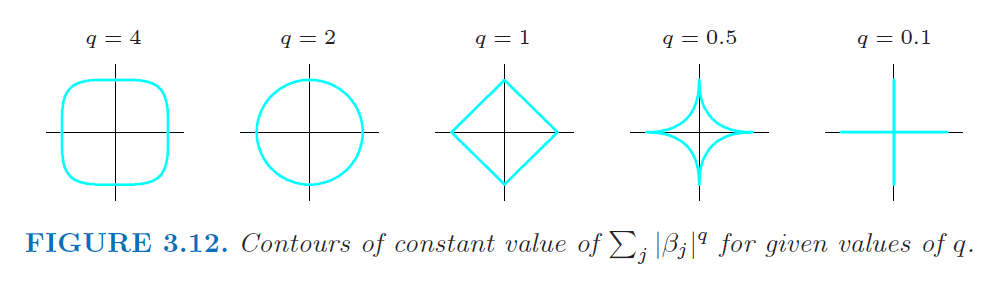
\includegraphics[scale=.4]{RegularizationContours}\\
To get 0's the function must not be differentiable at the axes
\end{frame}

\begin{frame}{Sparsity}
From: \emph{Elements of Statistical Learning} Hastie, Tibshirani, and Friedman\\
\bigskip
\begin{center}
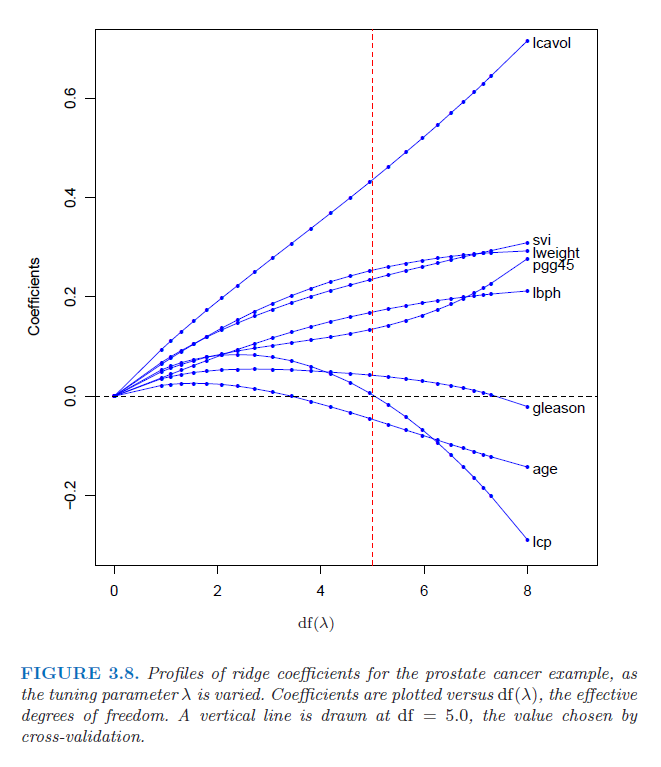
\includegraphics[scale=.26]{RidgeProfile}
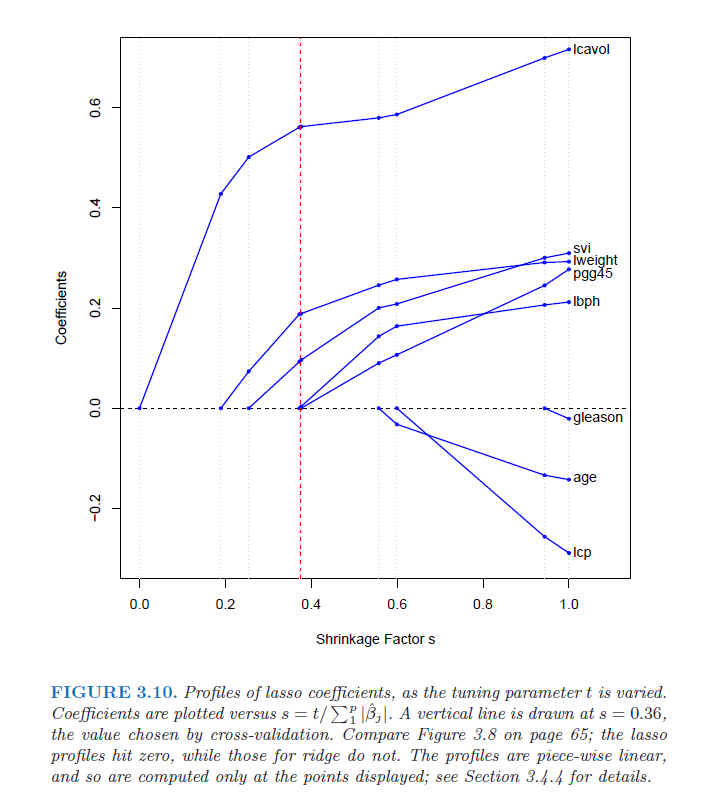
\includegraphics[scale=.25]{LassoProfile}\\
\end{center}
\end{frame}

\begin{frame}{Sparsity}
From: Regularization and Variable Selection via the Elastic Net (Zou and Hastie 2005)\\
\begin{center}
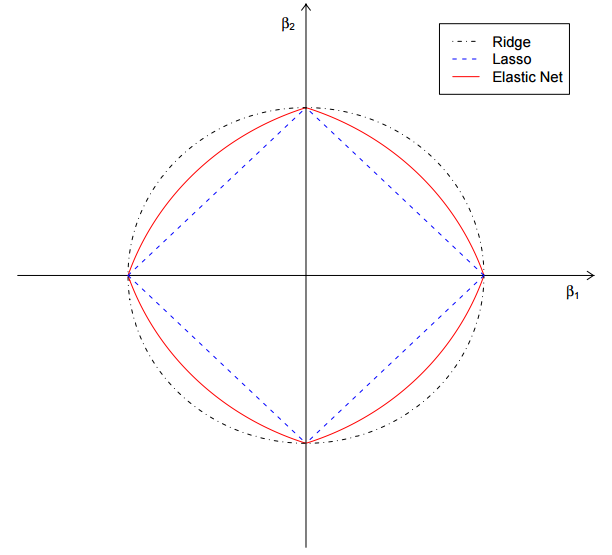
\includegraphics[scale=.35]{RidgevElasticvLASSO}\\
\end{center}
Elastic net regularization represents a compromise between LASSO and Ridge.
\end{frame}

\begin{frame}{Cross-validation}
The penalty parameter, $\lambda$, is considered ``tuning" parameter.\\
How do we choose $\lambda$?
\pause
\bigskip
\begin{itemize}
\item Can be estimated from the data but this is generally not done.
\item Select $lambda$ based on prediction error using cross-validation
\end{itemize}
\end{frame}

\begin{frame}{Cross-validation}
K-fold Cross-validation steps:
\bigskip
For each value of $\lambda$
\begin{itemize}
\item[1.] Divide the data into two parts
\item[2.] ``Train" the model on the first data set
\item[3.] Predict the outcome for the data in the second and calculate the error
\item[4.] Repeat k times for each value of $\lambda $
\end{itemize}
\end{frame}

\begin{frame}{Cross-validation}
Find the $\lambda$ with the smallest prediction error and variance.\\
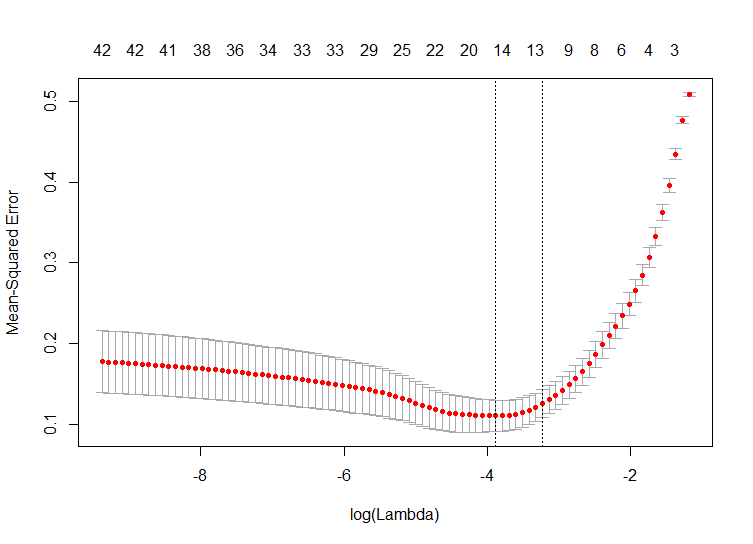
\includegraphics[scale=.38]{ExampleCVplot}\\
\end{frame}

\begin{frame}{Cross-validation}
What are some potential problems with this approach?
\bigskip
\pause
\begin{itemize}
\item Need a substantial amount of data.
\pause
\bigskip
\item Results may be very specific to the original data.
\pause
\bigskip
\item Interpretation of shrunken coefficients.
\end{itemize}
\end{frame}

\begin{frame}{LASSO Implementation}
\textbf{SAS:}\\
PROC GLMSELECT  SEED=123;  \\
PARTITION= ...;
MODEL= .../ SELECTION=LASSO ;\\
(or SELECTION=LAR)\\
RUN;\\

\smallskip
\hyperlink{https://www.youtube.com/watch?v=bWhJ9ixN8e0}{YouTube Tutorial (click here)}\\

\bigskip
\textbf{R:}\\
Package ``glmnet" (created by Trevor Hastie and Junyang Qian)\\
\smallskip
cv.glmnet(x=predictors, y=response, family="gaussian", alpha=1, nlambda=100, nfolds=k)\\
\smallskip
glmnet(x=predictors, y=response, family="gaussian", alpha=1, lambda=best.lambda)\\

\end{frame}

\section{Model Selection}

\begin{frame}{Model Selection}
Variable selection finds important variables but what if you want to find important \emph{relationships?}\\
\pause
Model Selection:
\begin{itemize}
\pause
\item Start with a set of \emph{plausible} models (must have some theory!)
\pause
\item Fit and rank the models using some Information Criteria
  \begin{itemize}
  \item AIC, BIC, KIC, AICc, qAIC....
  \end{itemize}
  \pause
\item Select the top ranked model \textbf{\emph{or}} Average the models to incorporate model selection uncertainty.
\end{itemize}
\end{frame}

\begin{frame}{Information Criteria}
All the information criteria follow the same general formula:\\
\bigskip
\begin{center}
.IC = -log(likelihood) + complexity penalty\\
\end{center}
\bigskip
\begin{itemize}
\item $AIC= 2k - 2ln(L)$
\item $BIC= -2ln(L) + k \cdot ln(n)$
\item $KIC = -2 \text{penalized log-likelihood} + C\left(\hat{\Sigma}_{\hat{\theta}}\right)$*
\end{itemize}
{\tiny *I won't subject you to this function!}
\end{frame}

\begin{frame}{Model Averaging}

\end{frame}

\begin{frame}{Questions?}


Stanford open course on statistical learning (you will learn R at the same time)

\end{frame}

\end{document}
